\documentclass[12pt]{article}
\usepackage{graphicx}
\usepackage {color}
\usepackage{pdfpages}
\usepackage{float}
\usepackage{changebar}
\usepackage{enumitem,amssymb}
\renewcommand{\familydefault}{\sfdefault}
\usepackage[margin=1.2in]{geometry}
\usepackage{graphicx}
\usepackage{wrapfig}
\usepackage[super]{cite}
\usepackage{subcaption}
\usepackage[table]{xcolor}
\usepackage{amsmath}
\usepackage[sort, numbers]{natbib}
\usepackage{multirow}
\usepackage{tabularx}
\usepackage{siunitx}
\usepackage{matlab-prettifier}
\usepackage{wrapfig,lipsum,booktabs}
%%%%%%%%%%%%Defining the margins %%%%%%%%%%%%%%%%%%%%%
\textheight 9.in
\textwidth 6.5in
\topmargin -.5in
\oddsidemargin 0in
\setlength{\parskip}{\smallskipamount}

%%%%%%%%%%%%%%Specific Commands %%%%%%%%%%%%%%%%%%
\newcommand{\eg}{{\em e.g.,}}
\newcommand{\ie}{{\em i.e.,}}
\newcommand{\etc}{{\em etc.,}}
\newcommand{\etal}{{\em et al.}}
\newcommand{\degrees}{{$^{\circ}$}}
\newcommand{\fig}[1]{\textbf{Figure #1}}

%%%%%%%%%%%%%%%%%%%%%%%%%%%% Setting to control figure placement
% These determine the rules used to place floating objects like figures 
% They are only guides, but read the manual to see the effect of each.
\renewcommand{\topfraction}{.9}
\renewcommand{\bottomfraction}{.9}
\renewcommand{\textfraction}{.1}
\renewcommand{\familydefault}{\sfdefault} %setting the san serif font

%%%%%%%%%%%%%%%%%%%%%%%% Line spacing
% Use the following command for ``double'' spacing
%\setlength{\baselineskip}{1.2\baselineskip}
% and this one for an acceptable NIH spacing of 6lpi based on 11pt
%\setlength{\baselineskip}{.9\baselineskip}
% The baselineskip does not appear to work when we include a maketitle
% command in the main file.  Something there must set the line spacing
% If we use this next command, then things seem to work.
\renewcommand{\baselinestretch}{.9}

\setcounter{secnumdepth}{0} %make no numbers but have a table of contents


\begin{document}

\title{HW 4: Medical Imaging Systems}
\author{Jake Bergquist, u6010393 }
\maketitle

\section{Q1}
\noindent\textbf{a: } 
Attached is the drawn sinogram for (a). All of the profiles are either semicircular or semi oval with a smooth transition between the different angles.

\noindent\textbf{b: } 
Attached is the drawn sinogram for (b). All profiles have either a semicircle, or two, or some overlap of two. The 0 degree projection has double the peak intensity of any of the projections where the two semicircles do not overlap. One of the circles is closer to the center than the other leading to the kind of mirroring effect seen in the sinogram profile.

\noindent\textbf{c: }
Attached is the sinogram for (c). All profiles are either trapezoids, rectangles or triangles. Assuming a uniform diffusion coefficient the max intensity of the 45 degree projections (ones that cross the diagonal of the square perfectly) is $\sqrt{2}$ larger than the max intensity of the 0 or 90 degree projections (the ones that are parallel to the sides of the square). Here max intensity meaning the maximum projection on the sinogram which corresponds to the maximal attenuation of the X ray beam through the sample.

\section{Q2}
\noindent\textbf{a: } 
The predicted object for part (a) is attached. The pattern of a small rectangle profile with high intensity at 0 and a large rectangular profile with less intensity at 90 or -90 suggests an object like a rectangle that is wider on the 90 degree projections than the 0 degree. Additionally there is a triagle profile at some angle less than 45 degrees which is the angle at which the projection would pass directly along the diagonal of the rectangle.

\noindent\textbf{b: }
The drawn object prediction is attached. For this one there seems to be a circle of lower attenuation coefficient centered at the origin . The remaining profile looks like an ofset oval like shape along the y axis as shown.

\section{Q3}
\noindent\textbf{a: }
Below is my function. Figure~\ref{basic} shows the results of 0, 30 and 45 degree projections of a rectangualr profile.

\begin{figure}[H]
	
	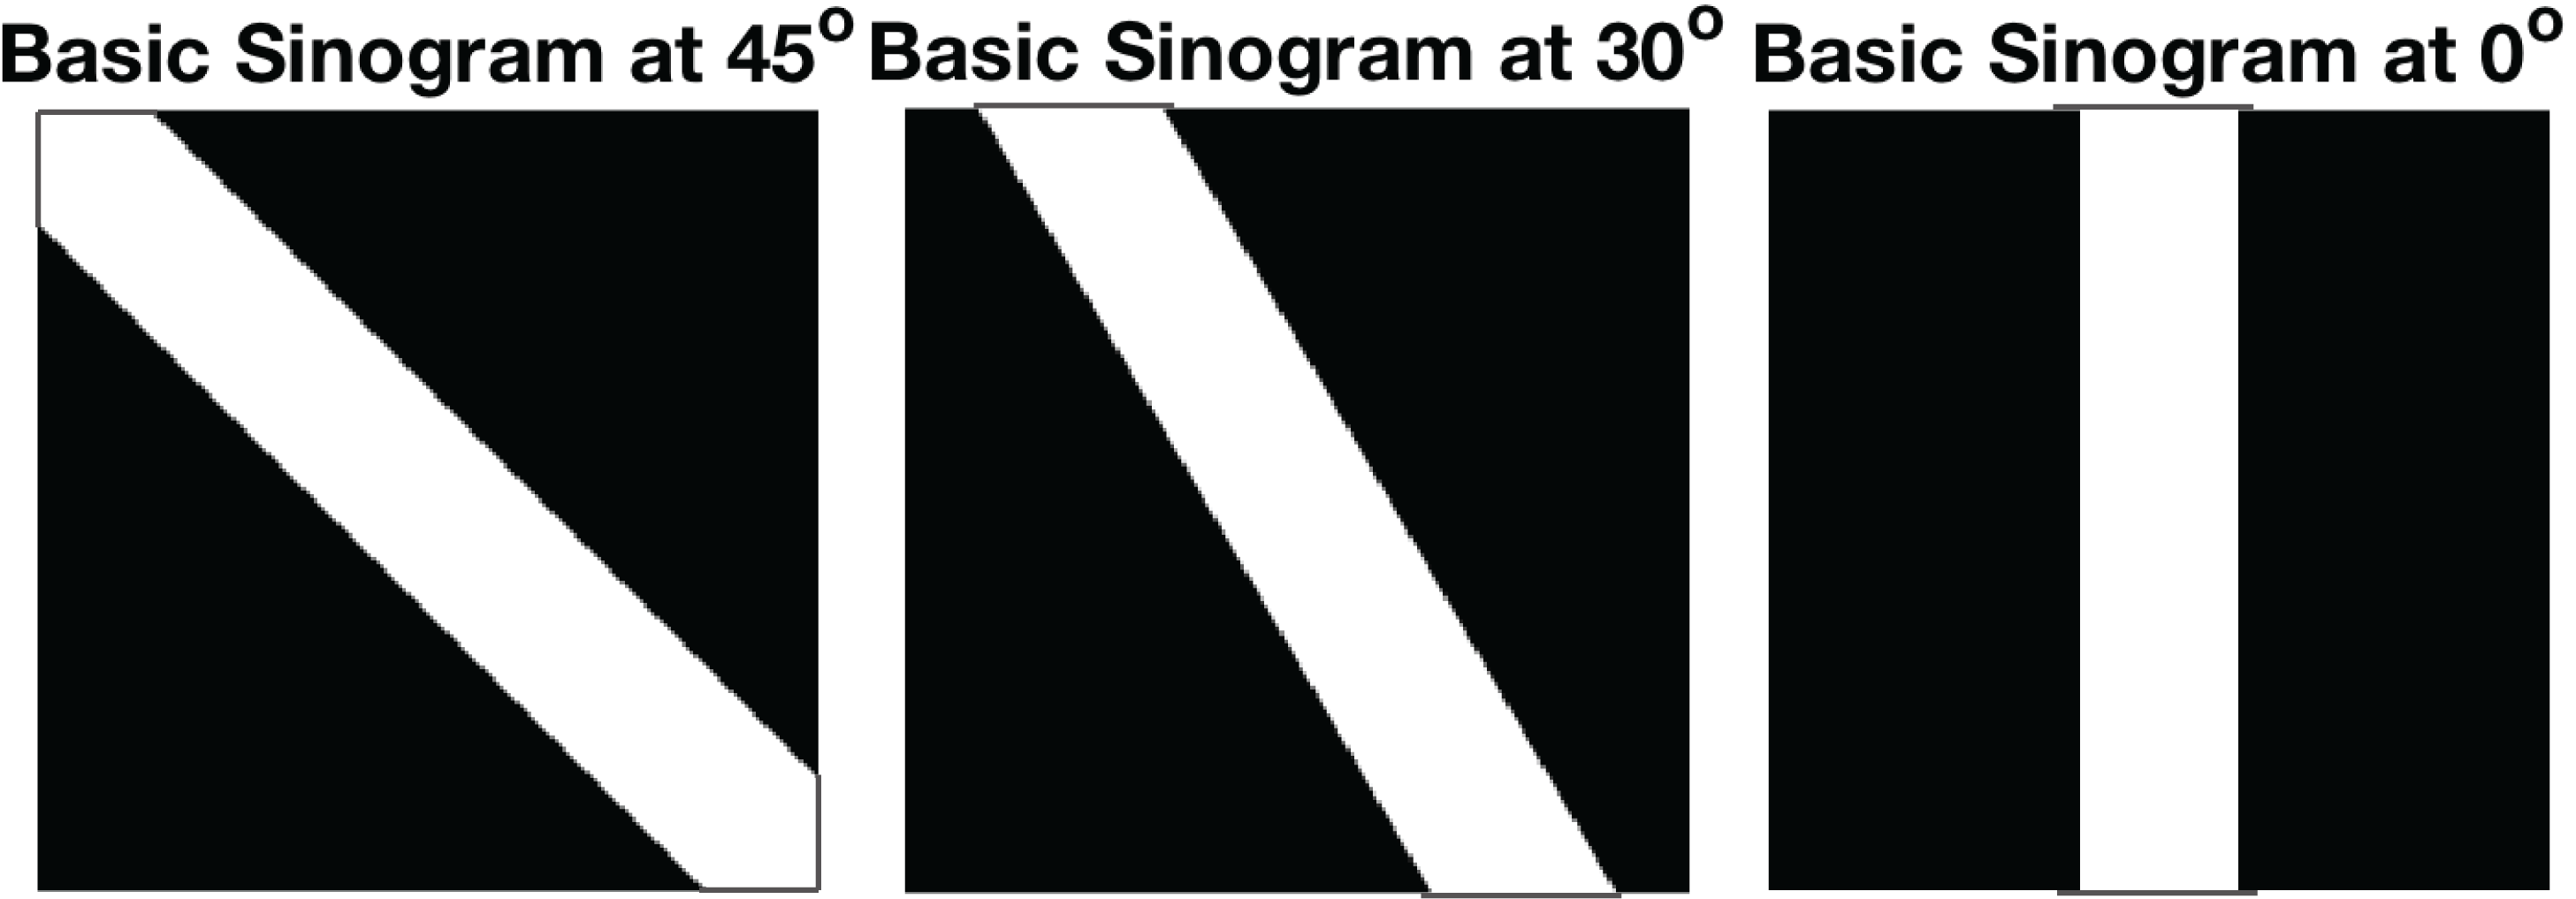
\includegraphics[width=\textwidth]{basicone.png}
	\caption{Basic sinogram projections for 0, 30, and 45 degrees for a rectangular profile.}
	\label{basic}
\end{figure}
\begin{lstlisting}[style=Matlab-editor]
function [Btheta] = BackPropSinogram(Rtheta,theta,interp)
%Input: Rtheta: the inogram projection at theta
%       Theta: the angle of the current projection
%       Interp: The interpolation method fromt eh fit function
%               Default: 'linearinterp'
%Assume image center is at the origin
%Assume Rtheta has an odd number of measurements

if ~exist(interp)
	interp = 'linearinter';
end


imageLim = floor(length(Rtheta)/2);
[X,Y] = meshgrid([-imageLim:imageLim],[imageLim:-1:-imageLim]);
RotCoords1 = Y.*sin(theta) + X.*cos(theta);
RotCoords2 = Y.*sin(pi/2-theta) + X.*cos(pi/2-theta);
Val = repmat(Rtheta,1,size(X,2));
sf = fit([X(:),Y(:)],Val(:),interp);
Btheta = sf(RotCoords2,RotCoords1);
Btheta(isnan(Btheta)) = 0;

%Below is the minimum line version of above (4 lines total)
%I chose to go with what is above because it is easier to read
%Both version produce the same output
%    [X,Y] = meshgrid([-floor(length(Rtheta)/2):floor(length(Rtheta)/2)],[floor(length(Rtheta)/2):-1:-floor(length(Rtheta)/2)]);
%    sf = fit([X(:),Y(:)],reshape(repmat(Rtheta,1,size(X,2)),[length(Rtheta)*size(X,2),1]),interp);
%    Btheta = sf(Y.*sin(pi/2-theta) + X.*cos(pi/2-theta),Y.*sin(theta) + X.*cos(theta));
%    Btheta(isnan(Btheta)) = 0;
end
\end{lstlisting}

\noindent\textbf{b: }
Figure~\ref{sino} shows the provided sinogram with 0, 90, and 180 degrees marked.
\begin{figure}[H]
	
	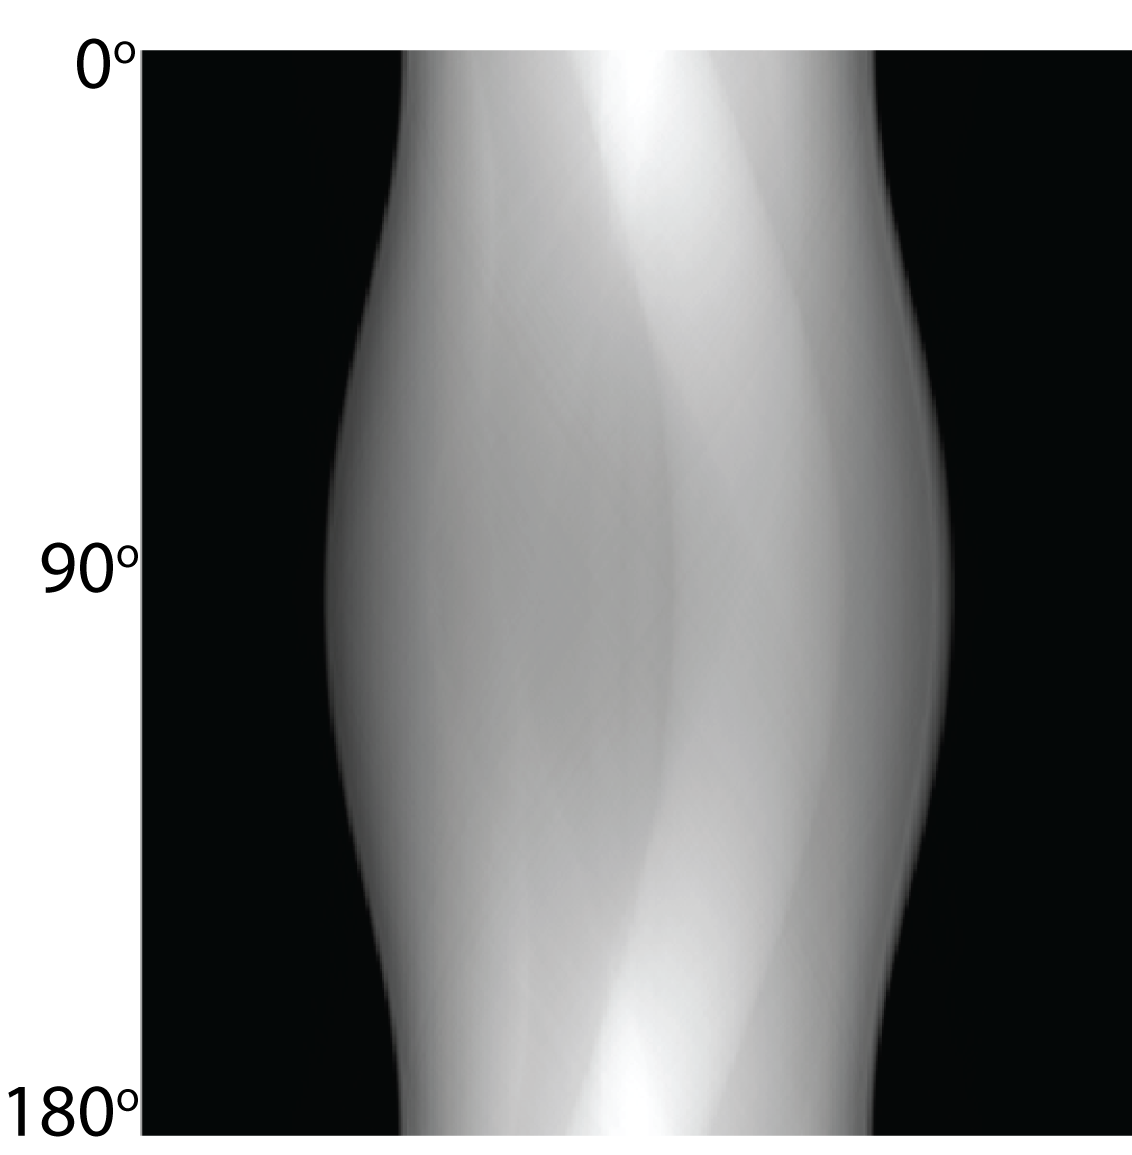
\includegraphics[width=\textwidth]{sinogram.png}
	\caption{Provided sinogram with 0, 90, and 180 degrees marked.}
	\label{sino}
\end{figure}

\noindent\textbf{c\&d: }
In Figure~\ref{direct} we see the results of backprojection. This is a very blurred image but we can barely make out that there seems to be some circular shape with perhaps another circle of different consistency within it. The Rho filtered results however are much clearer (Figure~\ref{rho}), where several detailed structures can be resolved. There are many more details such as different attenuation coefficients of material at teh border, several regions of large lower and higher attenuation and even some very small circles near the front that were completely unrecognizable in the direct backprojection results. The filter used is shown in Figure~\ref{filt} where the center point is the each of the sinogram profiles.
\begin{figure}[H]
	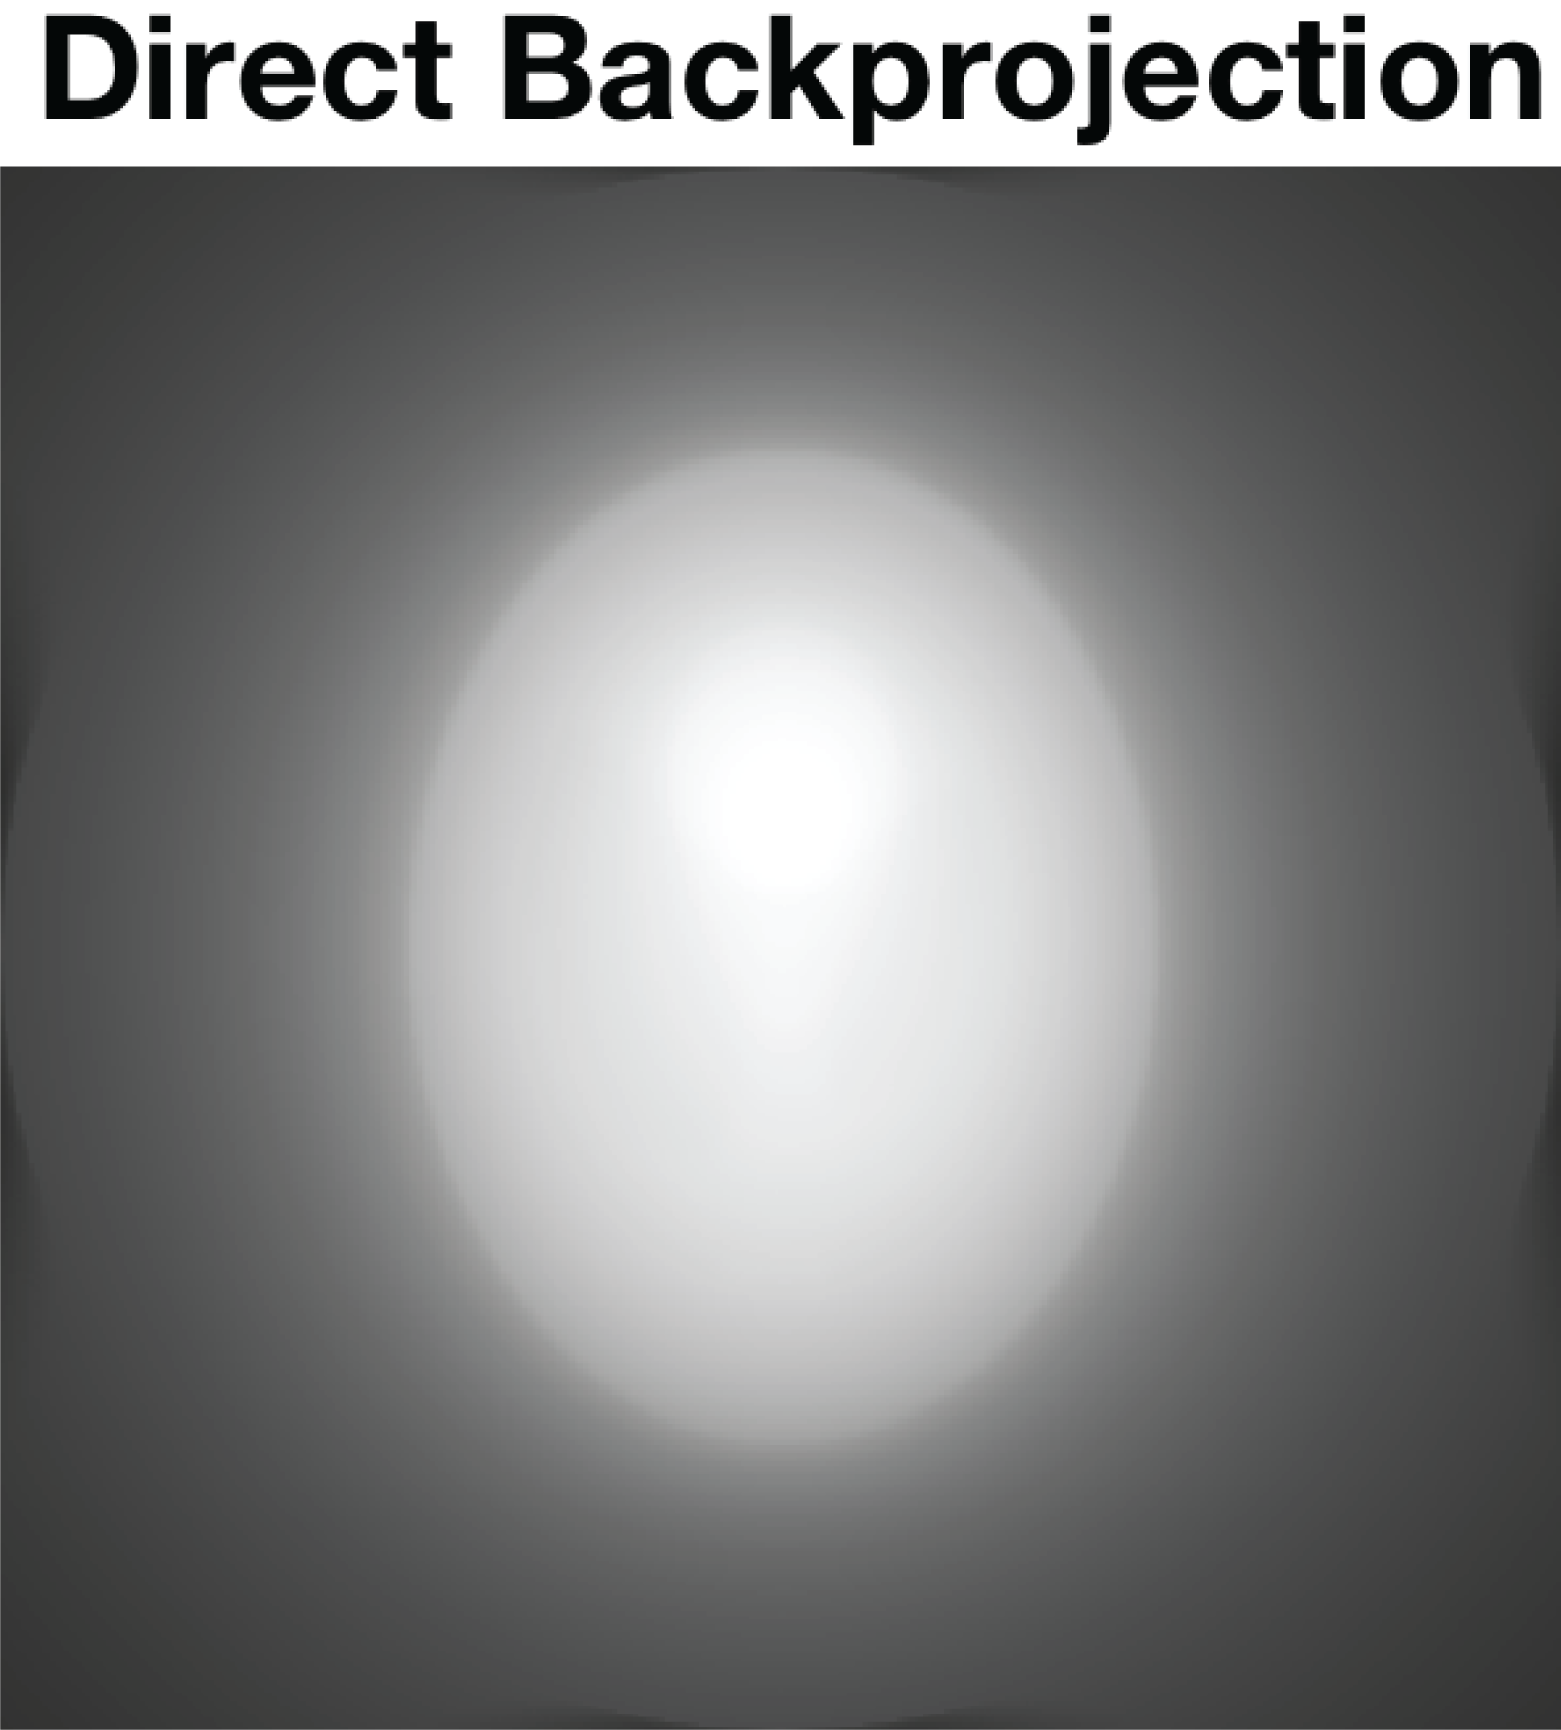
\includegraphics[width=\textwidth]{direct.png}
	\caption{Reconstructed image using direct backprojection.}
	\label{direct}
\end{figure}

\begin{figure}[H]
	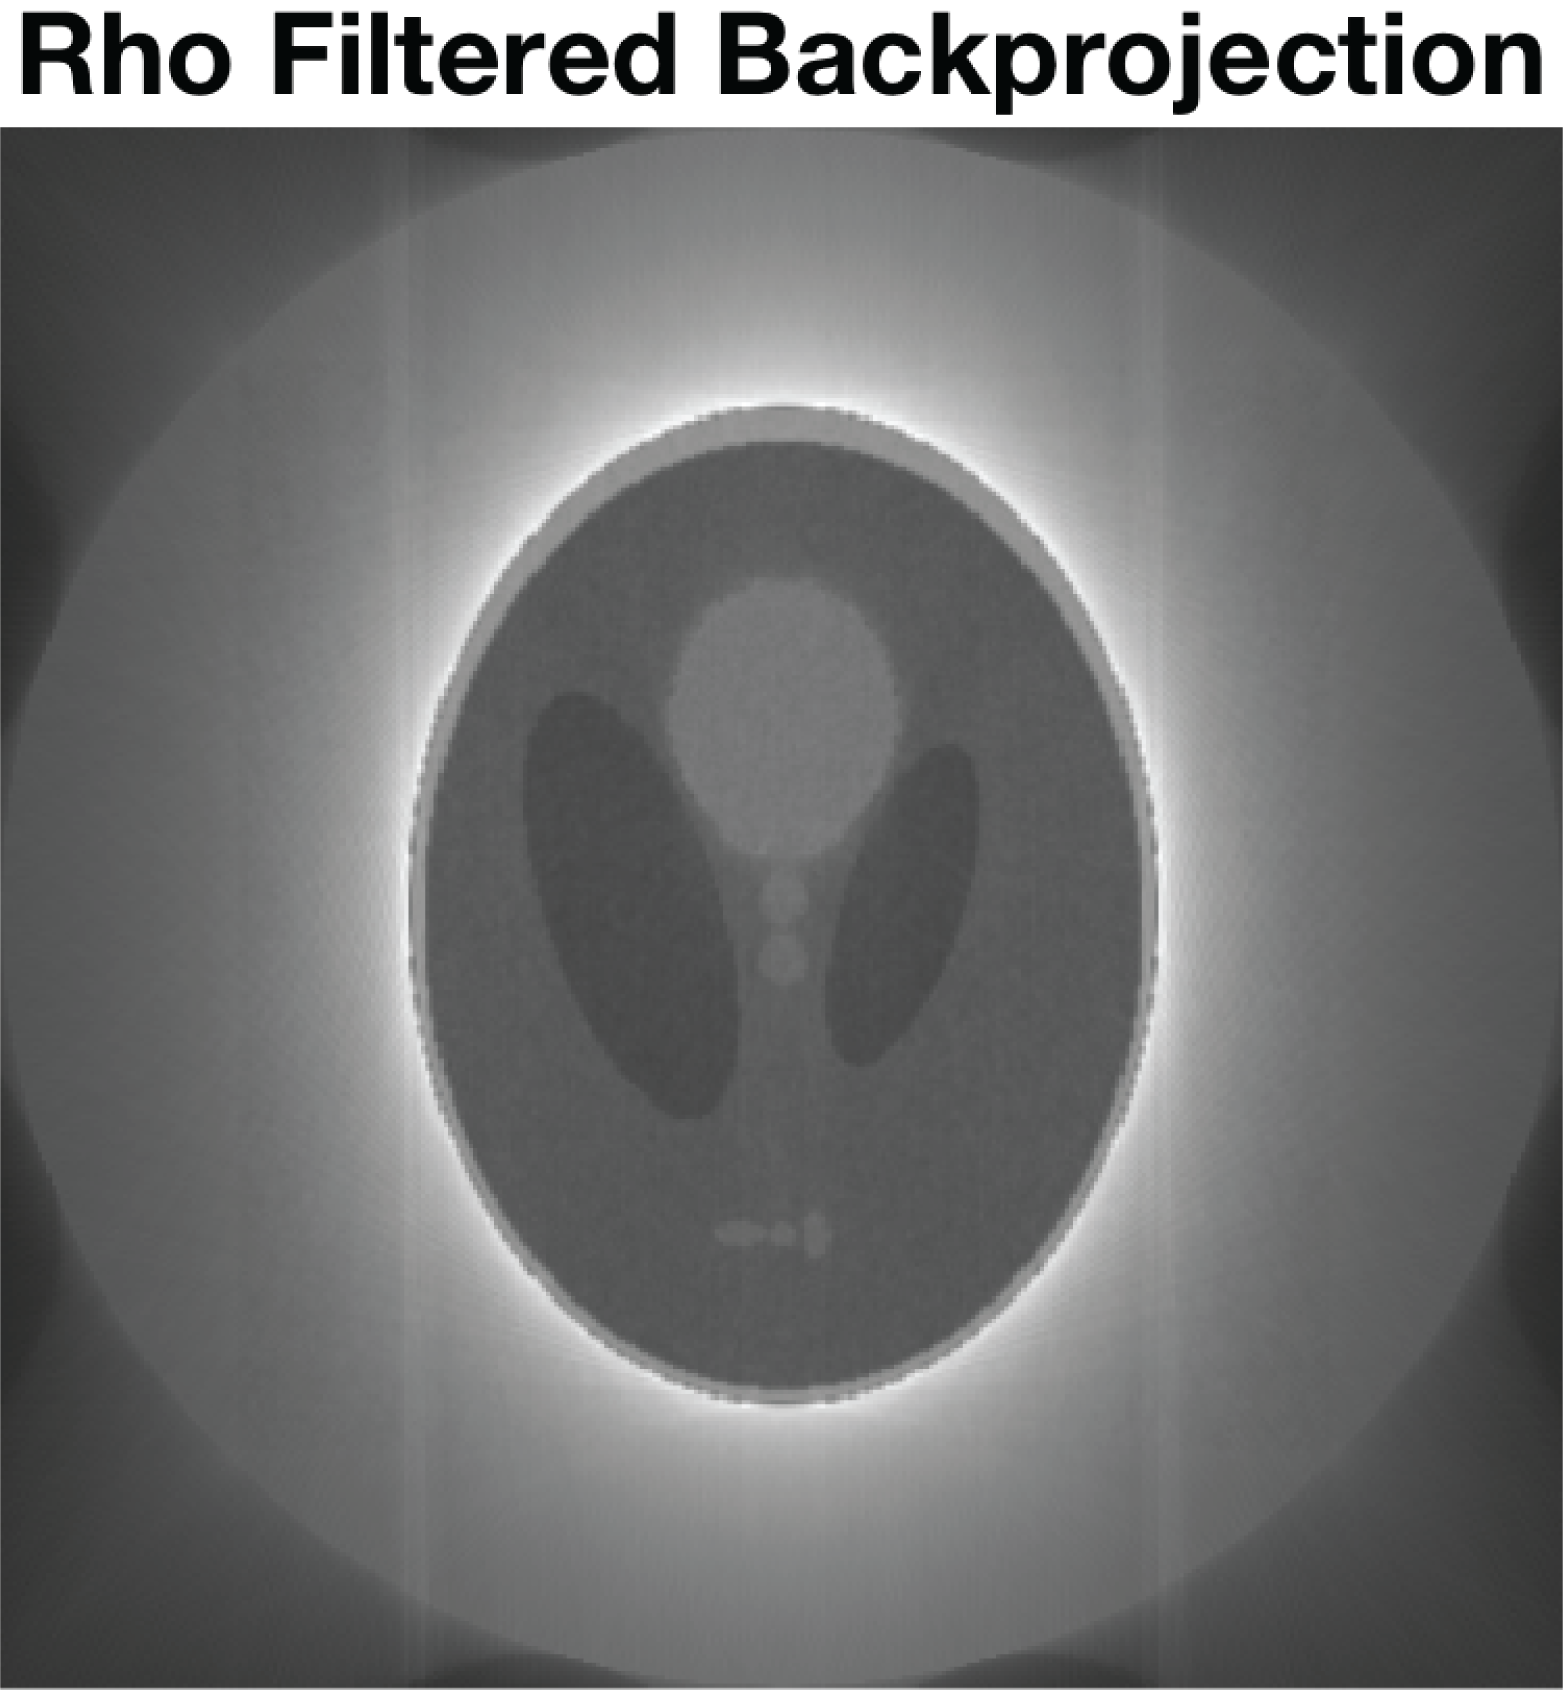
\includegraphics[width=\textwidth]{rhoFilt.png}
	\caption{Reconstructed image using Rho filtered backprojection.}
	\label{rho}
\end{figure}

\begin{figure}[H]
	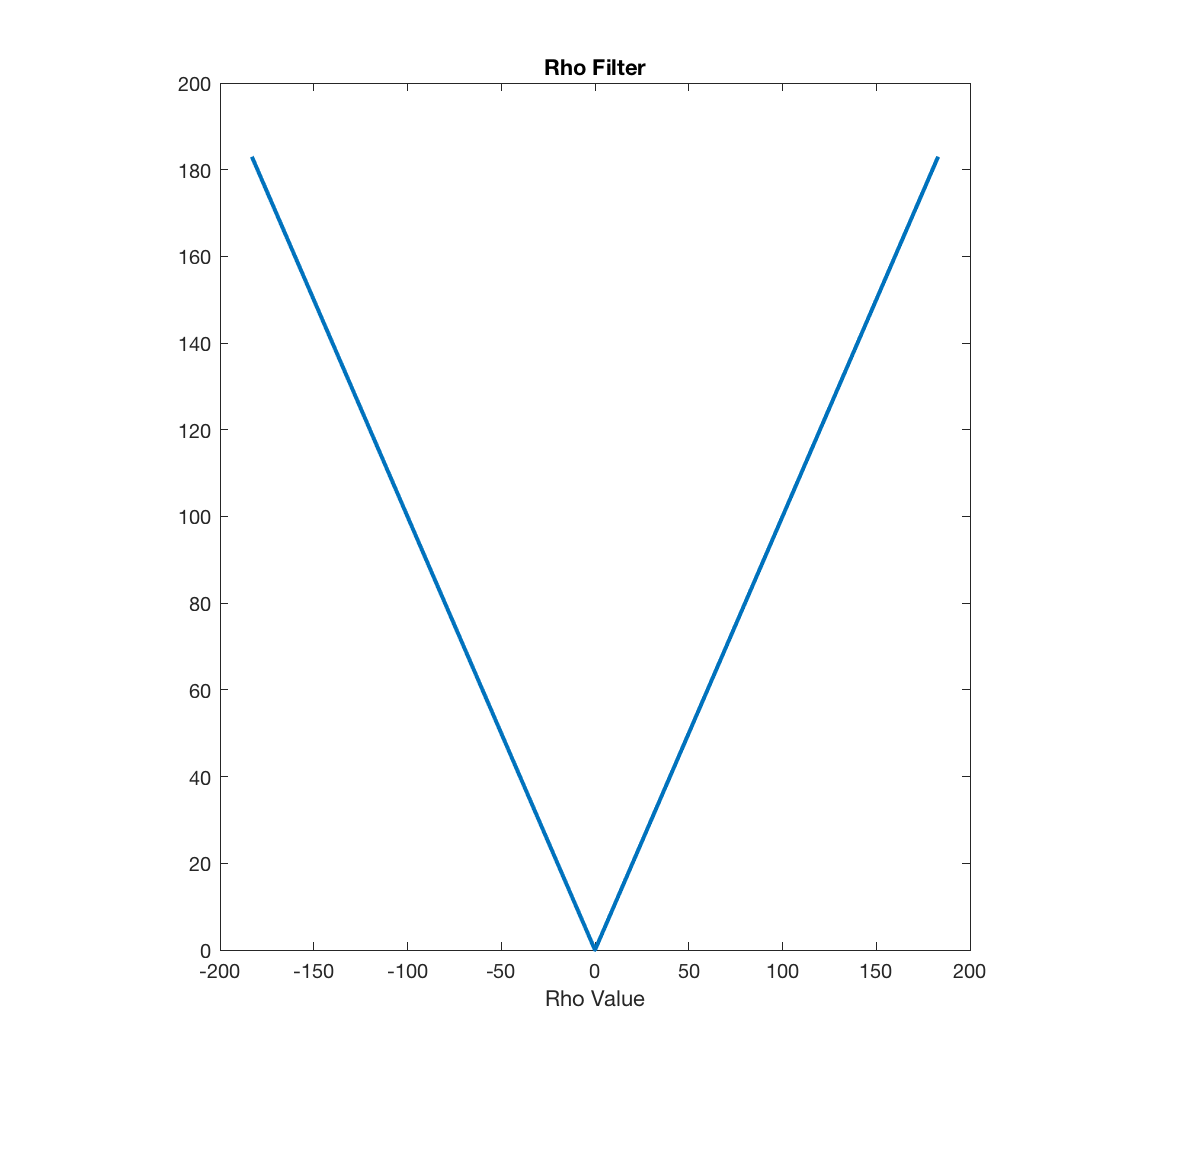
\includegraphics[width=\textwidth]{Filter.png}
	\caption{Filter used for Rho filtering.}
	\label{filt}
\end{figure}

\section{Q4}
The results of downsampling the number of projections (thetas) is shown in Figure~\ref{dtheta}. With this method of downsampling the number of pixels is not changed because the size of rho, the detector, is not affected. Thus the main artifact of this downsampling is projection artifact from fewer and fewer projections. This can be seen in a  sort of radial banding. More projections smooths out this effect.

By contrast the downsamlping of rho, the "number of detectors", causes the image to shrink and become more pixelated. This reduces the ability to resolve some of the smaller, closer together objects.

\begin{figure}[H]
	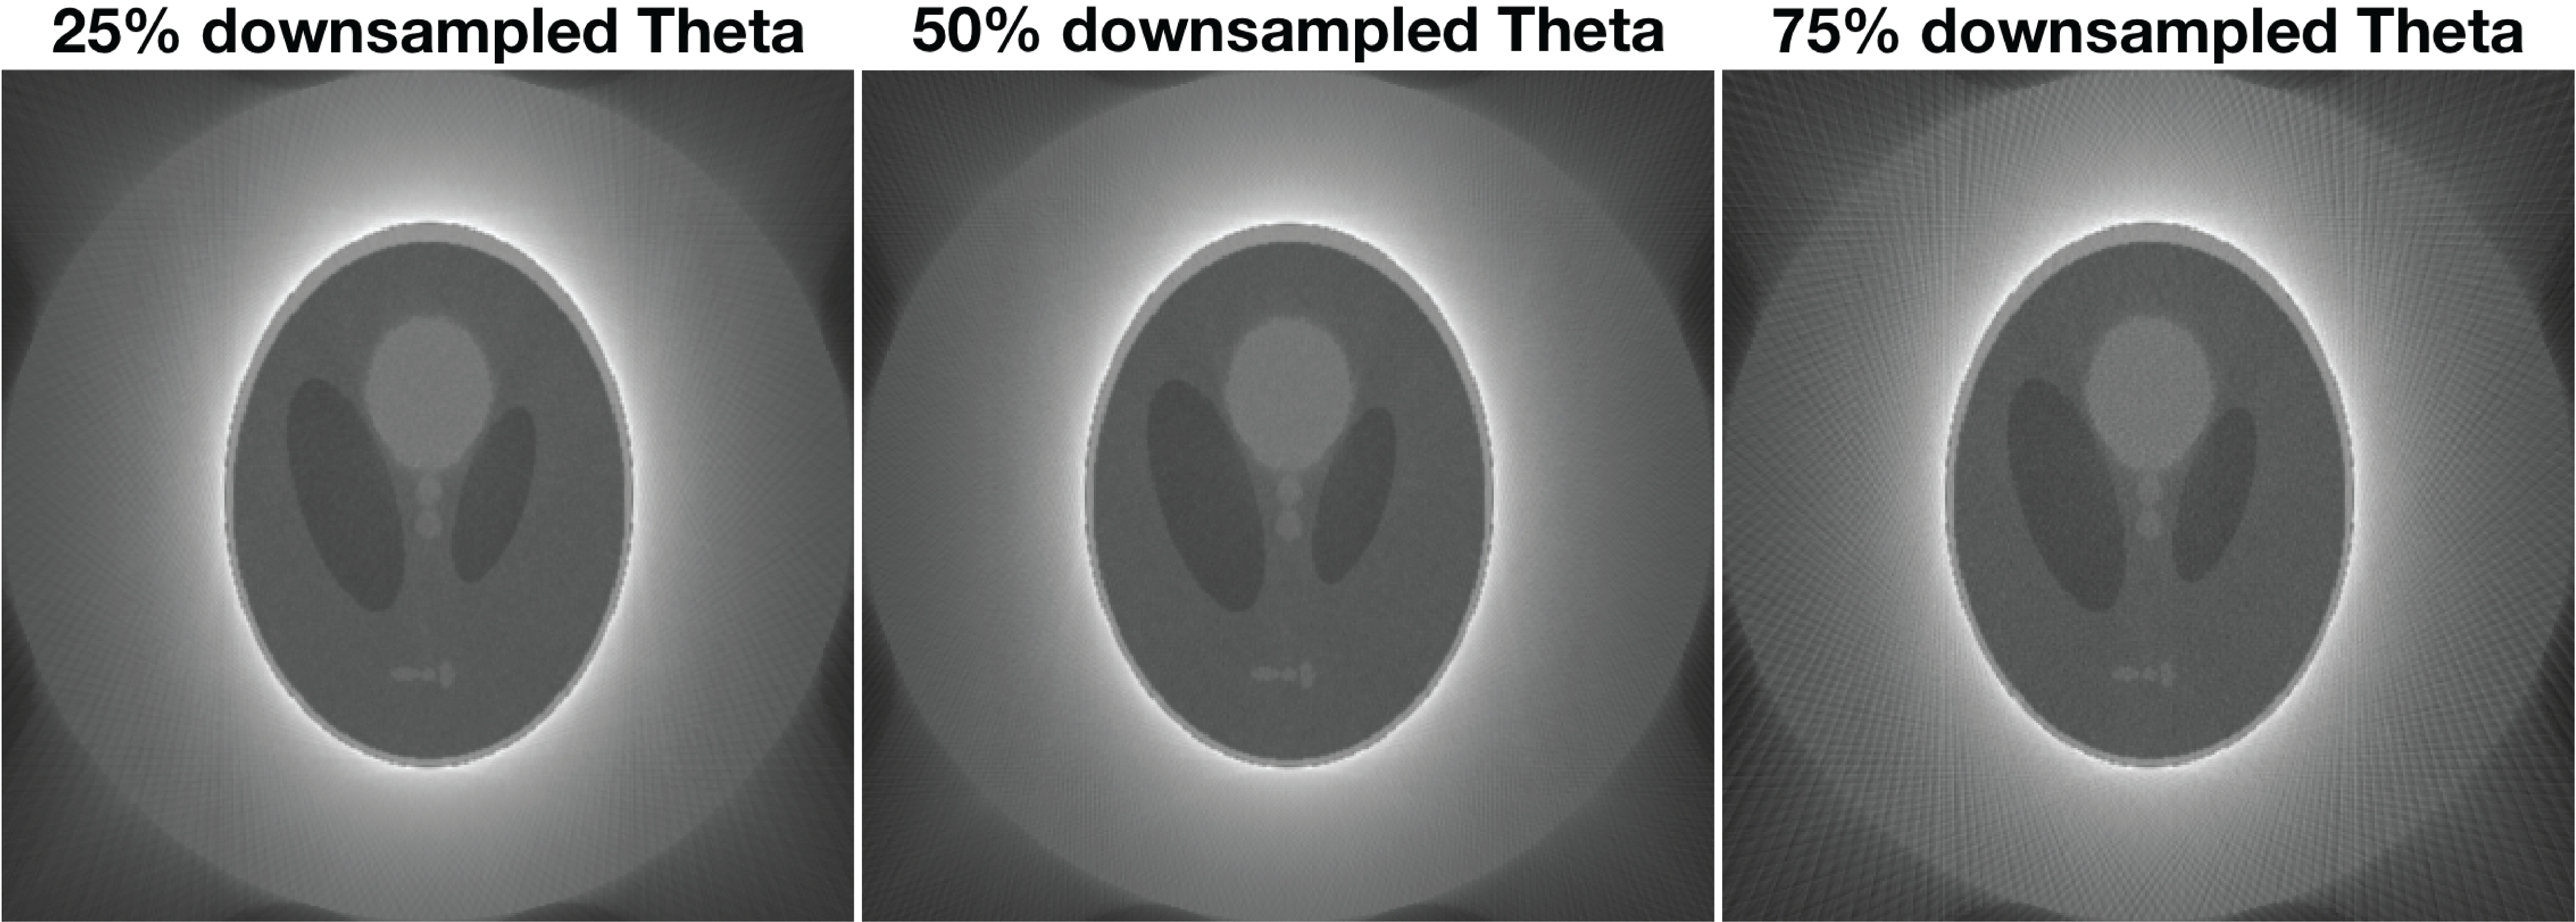
\includegraphics[width=\textwidth]{downtheta.png}
	\caption{Reconstructions using progressively more downsampled theta.}
	\label{dtheta}
\end{figure}
\begin{figure}[H]
	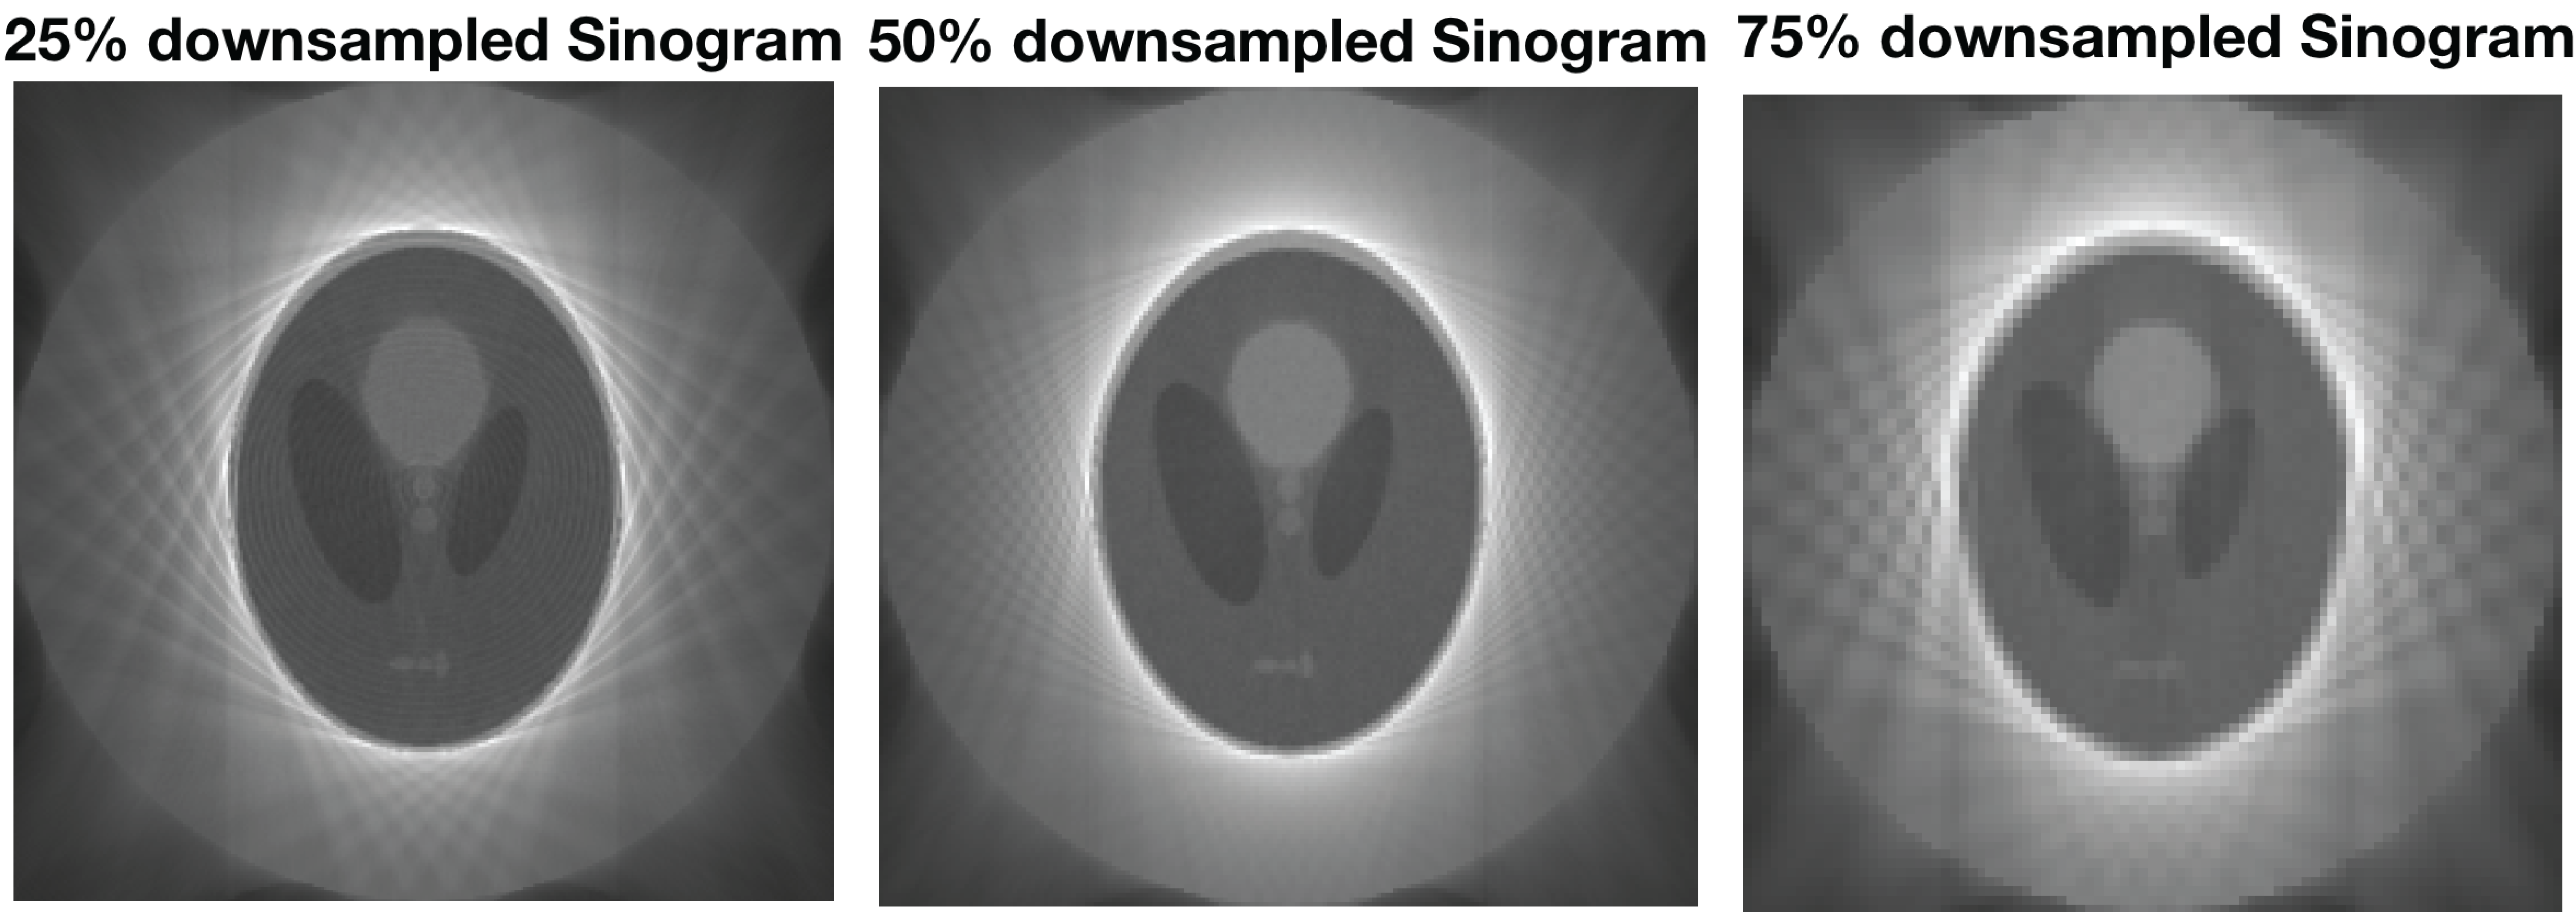
\includegraphics[width=\textwidth]{downrho.png}
	\caption{Reconstructions using progressively more downsampled rho.}
	\label{drho}
\end{figure}
\section{Q5}
Using the given values for water and air which should be at 0 and -1000 respctivly we can construct a mapping from emasured to tru Hounsfield number. In the form $T = am + b$ is a linear equation where $a$ is the "slope" and $b$ is the "y" intercept (here the Y axis is true values). Thus:\\
$
a = \frac{W_t - A_t}{W_o - A_o} = \frac{0 - -1000}{-20 - -1200} = \frac{1000}{1820} \approxeq 0.85\\
b = T - am = 0 - a*-20 = -16.95\\$

Now using these values we can solve for the true Hounsfield number for an observed value of 1850:\\
$T = am + b = 0.85 * 1850 - 16.95 = 1585\\$

 


\section{Appendix:}
Below is the matlab code used for this assignment to generate figures. Figures were post-processed and arranged in illustrator.
\begin{lstlisting}[style=Matlab-editor]
%%
clear
close all 
clc


%%
%Testing Backprojection

testThetas = deg2rad([0:5:175]);
simpleSinogram = zeros(201,1);
simpleSinogram(81:121,:) = 1;

t = 1;
figure(1);imshow(BackPropSinogram(simpleSinogram,testThetas(t),'linearinterp'));
title(sprintf('Basic Sinogram at %g^o',rad2deg(testThetas(t))));
set(gca,'fontsize',20)
t = 7;
figure(2);imshow(BackPropSinogram(simpleSinogram,testThetas(t),'linearinterp'));
title(sprintf('Basic Sinogram at %g^o',rad2deg(testThetas(t))));
set(gca,'fontsize',20)
t = 10;
figure(3);imshow(BackPropSinogram(simpleSinogram,testThetas(t),'linearinterp'));
title(sprintf('Basic Sinogram at %g^o',rad2deg(testThetas(t))));
set(gca,'fontsize',20)
[X,Y] = meshgrid(1:201,1:201);
b = zeros(length(simpleSinogram));
for t = 1:length(testThetas)
b = b + BackPropSinogram(simpleSinogram,testThetas(t),'linearinterp');
figure(4);imagesc(b./max(b(:)));title(sprintf('Proj %d',t));drawnow();
figure(5);surf(X,Y,b);zlim([0 40]);drawnow();
end



%%
b = zeros(length(simpleSinogram));
filter = abs([-floor(length(simpleSinogram)/2):floor(length(simpleSinogram)/2)])';
filteredSinogram = abs(ifft(fftshift(fft(simpleSinogram)).*filter));
for t = 1:length(testThetas)
b = b + BackPropSinogram(filteredSinogram,testThetas(t),'linearinterp');
figure(4);imagesc(b./max(b(:)));title(sprintf('Proj %d',t));drawnow();
figure(5);surf(X,Y,b);drawnow();
end

%%
figure(1);clf();
imshow(sinogram'/max(sinogram(:)))
%%
%Direct Backprojection
b = zeros(size(sinogram,1));
for t = 1:length(thetas)
b = b+BackPropSinogram(sinogram(:,t),deg2rad(thetas(t)),'linearinterp');
figure(1);imshow(b/max(b(:)));title(sprintf('Proj %d',t));drawnow();
end
figure(1);title('Direct Backprojection');set(gca,'fontsize',25)
%%
%Rho filtering
b = zeros(size(sinogram,1));
numSamples = size(sinogram,1);
rho = abs([-floor(numSamples/2):floor(numSamples/2)])';
Ft = fftshift(fft(sinogram),1);
M = abs(ifft(Ft.*rho));
%%
for t = 1:length(thetas)
b = b+BackPropSinogram(M(:,t),deg2rad(thetas(t)),'linearinterp');
figure(1);imshow(b/max(b(:)));title(sprintf('Proj %d',t));drawnow();
end
figure(1);title('Rho Filtered Backprojection');set(gca,'fontsize',25)
%%
%downsampling
%25% downsampled, skip every 4th angle
skipInds = [1:4:length(thetas)];
thetaInds = setdiff([1:length(thetas)],skipInds);
downSampleTheta = thetas(thetaInds);

b = zeros(size(sinogram,1));
for t = 1:length(downSampleTheta)
b = b+BackPropSinogram(M(:,thetaInds(t)),deg2rad(downSampleTheta(t)),'linearinterp');
figure(1);imshow(b/max(b(:)));title(sprintf('Proj %d',t));drawnow();
end
figure(1);title('25% downsampled Theta');set(gca,'fontsize',25)

%50% downsampeld uses every other
downSampleTheta = thetas(1:2:end);
thetaInds = [1:2:length(thetas)];
b = zeros(size(sinogram,1));
for t = 1:length(downSampleTheta)
b = b+BackPropSinogram(M(:,thetaInds(t)),deg2rad(downSampleTheta(t)),'linearinterp');
figure(2);imshow(b/max(b(:)));title(sprintf('Proj %d',t));drawnow();
end
figure(2);title('50% downsampled Theta');set(gca,'fontsize',25)
%75% downsampled uses every 4th 

downSampleTheta = thetas(1:4:end);
thetaInds = [1:4:length(thetas)];
b = zeros(size(sinogram,1));
for t = 1:length(downSampleTheta)
b = b+BackPropSinogram(M(:,thetaInds(t)),deg2rad(downSampleTheta(t)),'linearinterp');
figure(3);imshow(b/max(b(:)));title(sprintf('Proj %d',t));drawnow();
end
figure(3);title('75% downsampled Theta');set(gca,'fontsize',25)
%%
%Downsample sinogram
%25%
skipInds = [1:4:size(sinogram,1)];
sinogramInds = setdiff([1:size(sinogram,1)],skipInds);
downsampleSinogram = sinogram(sinogramInds,:);
downsampleSinogram = abs(ifft((fftshift(fft(downsampleSinogram),1).*abs([-floor(size(downsampleSinogram,1)/2):floor(size(downsampleSinogram,1)/2)]'))));
b = zeros(size(downsampleSinogram,1));
for t = 1:length(thetas)
b = b+BackPropSinogram(downsampleSinogram(:,t),deg2rad(thetas(t)),'linearinterp');
figure(1);imshow(b/max(b(:)));title(sprintf('Proj %d',t));drawnow();
end
figure(1);title('25% downsampled Sinogram');set(gca,'fontsize',25)

%50%
sinogramInds = [1:2:size(sinogram,1)-1];
downsampleSinogram = sinogram(sinogramInds,:);
downsampleSinogram = abs(ifft((fftshift(fft(downsampleSinogram),1).*abs([-floor(size(downsampleSinogram,1)/2):floor(size(downsampleSinogram,1)/2)]'))));
b = zeros(size(downsampleSinogram,1));
for t = 1:length(thetas)
b = b+BackPropSinogram(downsampleSinogram(:,t),deg2rad(thetas(t)),'linearinterp');
figure(2);imshow(b/max(b(:)));title(sprintf('Proj %d',t));drawnow();
end
figure(2);title('50% downsampled Sinogram');set(gca,'fontsize',25)


%75%
sinogramInds = [1:4:size(sinogram,1)-3];
downsampleSinogram = sinogram(sinogramInds,:);
downsampleSinogram = abs(ifft((fftshift(fft(downsampleSinogram),1).*abs([-floor(size(downsampleSinogram,1)/2):floor(size(downsampleSinogram,1)/2)]'))));
b = zeros(size(downsampleSinogram,1));
for t = 1:length(thetas)
b = b+BackPropSinogram(downsampleSinogram(:,t),deg2rad(thetas(t)),'linearinterp');
figure(3);imshow(b/max(b(:)));title(sprintf('Proj %d',t));drawnow();
end
figure(3);title('75% downsampled Sinogram');set(gca,'fontsize',25)
%%
%Hounsfield number fitting
water = [-20,0];
air = [-1200,-1000];

a = (water(2)-air(2))/(water(1)-air(1));
b = water(2)-a*water(1);

MysteryItem(1)=1850;
MysteryItem(2) = a*MysteryItem(1) + b;

figure(1);clf();
hold on;
scatter([water(1),air(1),MysteryItem(1)],[water(2),air(2),MysteryItem(2)]);
plot([-1300:1900],a.*[-1300:1900]+b);

\end{lstlisting}

\end{document}



\begin{figure}[H]
	\centering
	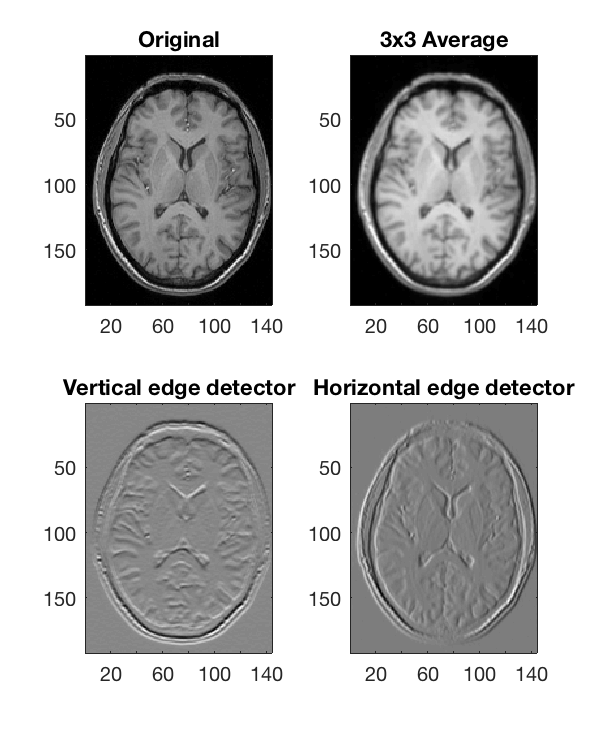
\includegraphics[width=\textwidth]{Figures/convs.png}
	\caption{}
	\label{Fig:conv}
\end{figure}

\begin{lstlisting}[style=Matlab-editor]

\end{lstlisting}




